% VUT FIT MITAI
% MSZ 2021/2022
% Author: Vladimir Dusek
% Login: xdusek27

%%%%%%%%%%%%%%%%%%%%%%%%%%%%%%%%%%%%%%%%%%%%%%%%%%%%%%%%%%%%%%%%%%%%%%%%%%%%%%%%

% Path to figures
\graphicspath{{upa/porozumeni_datum/figures}}

%%%%%%%%%%%%%%%%%%%%%%%%%%%%%%%%%%%%%%%%%%%%%%%%%%%%%%%%%%%%%%%%%%%%%%%%%%%%%%%%

\chapter{UPA~--~Porozumění datům (důvod a cíl; popisné charakteristiky dat a vizualizační techniky; korelační analýza).}

%%%%%%%%%%%%%%%%%%%%%%%%%%%%%%%%%%%%%%%%%%%%%%%%%%%%%%%%%%%%%%%%%%%%%%%%%%%%%%%%

\section{Zdroje}

\begin{compactitem}
    \item \path{11-porozumeni_datum.pdf}
    \item \path{UPA_2019-12-03.mp4}
    \item \path{UPA_2019-12-10.mp4}
\end{compactitem}

%%%%%%%%%%%%%%%%%%%%%%%%%%%%%%%%%%%%%%%%%%%%%%%%%%%%%%%%%%%%%%%%%%%%%%%%%%%%%%%%

\section{Důvod a cíl porozumění datům}

\begin{compactitem}
    \item Druhý krok modelu procesu CRISP.

    \item Cílem je získat detailní informace o datech, jejich vlastnostech a vytvořit podklady pro datovou sadu. Dozvědět se o datech co nejvíce.

    \item Předpoklady (z pohledu dat): \begin{compactitem}
        \item chápeme problematiku (máme kontext),
        \item máme stanovený cíl projektu a kritéria úspěšnosti,
        \item víme, jaká data jsou / budou k dispozici,
        \item víme, o jakou DM úlohu půjde.
    \end{compactitem}

    \item Vstup: \begin{compactitem}
        \item Dostupné datové zdroje a dokumentace k nim.
    \end{compactitem}

    \item Výstup: \begin{compactitem}
        \item Podklady pro vytvoření počáteční datové sady nebo přímo vytvoření.
        \item Detailní informace o vlastnostech dat (popisné charakteristiky + grafy).
    \end{compactitem}

    \item Dosažením cíle zahrnuje kroky: \begin{compactitem}
        \item Rozpracovaní informace -- Jaké data máme, význam, dostupnost, cena, věrohodnost dat.

        \item Popis dat -- struktura, význam, formát a množství dat.

        \item Prozkoumání dat (explorační analýza) -- popisné charakteristiky, grafy, korelace, \dots

        \item Zhodnocení kvality dat -- Úplnost, chybějíci hodnoty, šum, \dots
    \end{compactitem}
\end{compactitem}

%%%%%%%%%%%%%%%%%%%%%%%%%%%%%%%%%%%%%%%%%%%%%%%%%%%%%%%%%%%%%%%%%%%%%%%%%%%%%%%%

\section{Popisné charakteristiky z hlediska distribuce výpočtu}

\begin{compactitem}
    \item \textbf{Distributivní} \begin{compactitem}
        \item Lze počítat distribuovaně.
        \item Např.: počet prvků.
    \end{compactitem}

    \item \textbf{Algebratické} \begin{compactitem}
        \item Výsledek je algebraická operace nad mezivýsledky, které lze počítat distribuovaně.
        \item Např.: průměr.
    \end{compactitem}

    \item \textbf{Holistické} \begin{compactitem}
        \item Lze spočítat pouze výpočtem nad celým souborem.
        \item Např.: medián.
    \end{compactitem}
\end{compactitem}

%%%%%%%%%%%%%%%%%%%%%%%%%%%%%%%%%%%%%%%%%%%%%%%%%%%%%%%%%%%%%%%%%%%%%%%%%%%%%%%%

\section{Statistické popisné charakteristiky}

\begin{compactitem}
    \item Různými statistickými metodami se snažíme datům lépe porozumnět a získat o nich více informací.
\end{compactitem}

\begin{compactitem}
    \item \textbf{Míry polohy} -- Určují střed dat, případně další body z hlediska hodnot dat. \begin{compactitem}
        \item Aritmetický průměr (vážený průměr, citlivost na odlehlé hodnoty)

        \item Geometrický průměr (n-tá odmocina ze součinu hodnot, kde n je počet vzorků). Typicky pro výpočet tempa růsta.

        \item Harmonický průměr -- Počet vzorků / suma převrácených hodnot.

        \item Medián

        \item Modus

        \item Kvantily \begin{compactitem}
            \item Má 2 parametry $(k, q)$, $q$-kvantilů rozděluje uspořádaný datový soubor na $q$ přibližně stejně pravděpodobných intervalů (stejný počet výskytu).
            \item Hodnoty kvantilů jsou hodnoty náhodné veličiny, tedy průměr v každém $q$ intervalu.
            \item Pro $q = 100$ percentily, $q = 10$, decily, $q = 5$ kvintily, $q = 4$ kvartily.
        \end{compactitem}
    \end{compactitem}

    \item \textbf{Míry variability} -- Určují rozptýlenost hodnot kolem středu. \begin{compactitem}
        \item Rozpětí -- max-min, ovlivněno extrémy
        \item Mezikvartilové rozpětí -- rozpětí 50\,\% středních hodnot, např. pro kvartil, $q_3$ -- $q_2$
        \item Rozptyl
        \item Směrodatná odchylka
    \end{compactitem}

    \item \textbf{Další} \begin{compactitem}
        \item šikmost, špičatost, \dots
    \end{compactitem}

\end{compactitem}

%%%%%%%%%%%%%%%%%%%%%%%%%%%%%%%%%%%%%%%%%%%%%%%%%%%%%%%%%%%%%%%%%%%%%%%%%%%%%%%%

\section{Vizualizační techniky}

\subsection{Vizualizační technika pro jeden atribut}

\begin{compactitem}
    \item Cíl -- ukázat rozložení hodnot atributu.

    \item Pro kvantitativní atributy -- krabicový graf, graf hustoty pravděpodobnosti, houslový graf, kvantilový graf, \dots

    \item Pro kategorické atributy -- histogram.
\end{compactitem}

\subsection{Vizualizační technika pro více atributů}

\begin{compactitem}
    \item Cíl: \begin{compactitem}
        \item Porovnání rozložení hodnot.

        \item Odhalení potenciálních vztahů mezi atributy (korelace).
    \end{compactitem}

    \item Porovnání rozložení hodnot dvou atributů: \begin{compactitem}
        \item krabicový / houslový graf,
        \item histogram,
        \item bodový graf, lokální regrese.
    \end{compactitem}

    \item Porovnání hodnot více atributů: \begin{compactitem}
        \item krabicový / houslový graf,
        \item matice grafů,
        \item rozšíření použití hloubky, barvy, velikosti, tvaru, \dots,
        \item systém paralelních souřadnic.
    \end{compactitem}
\end{compactitem}

\subsection{Konkrétní typy vizualizací}

\subsubsection{Krabicový graf (box plot)}

\begin{compactitem}
    \item Rozdělení podle kvartilů.
    \item Zobrazen medián, odlehlé hodnoty (1. a 4. kvartil) a maximum i minimum.
    \item Na ose x máme kategorický atribut, na ose y kvantitativní atribut.
\end{compactitem}

\begin{figure}[H]
    \centering
    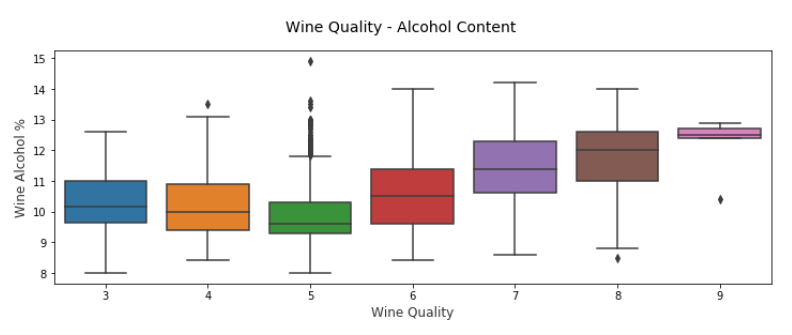
\includegraphics[width=1\linewidth]{box_plot.png}
    \caption{Krabicový graf.}
\end{figure}

\subsubsection{Histogram, graf hustoty pravděpodobnosti}

\begin{figure}[H]
    \centering
    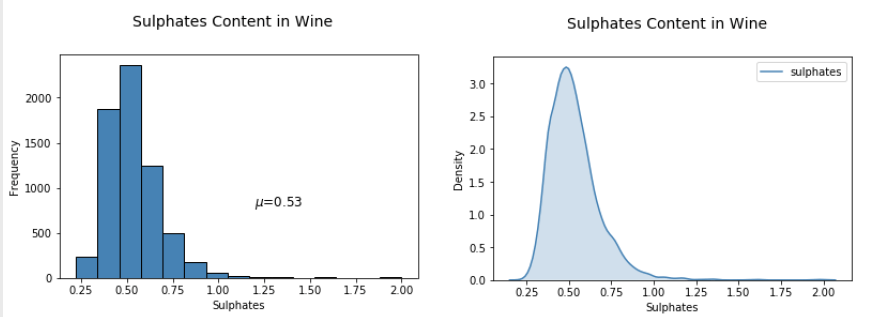
\includegraphics[width=1\linewidth]{histogram_density.png}
    \caption{Histogram a graf hustoty pravděpodobnosti.}
\end{figure}

\subsubsection{Houslový graf}

\begin{compactitem}
    \item Kombinace krabicového grafu a grafu hustoty.
    \item Dokáže odhalit vícemodální data! (viz obrázek, více než jeden vrchol)
\end{compactitem}

\begin{figure}[H]
    \centering
    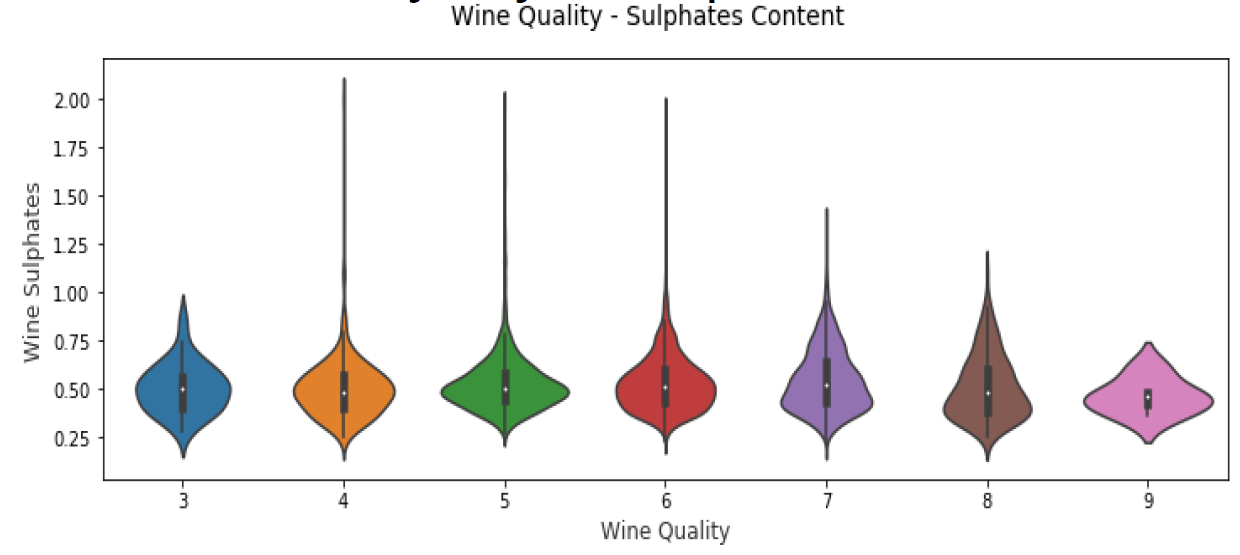
\includegraphics[width=1\linewidth]{houslovy_graf_1.png}
    \caption{Houslový graf 1.}
\end{figure}

\begin{figure}[H]
    \centering
    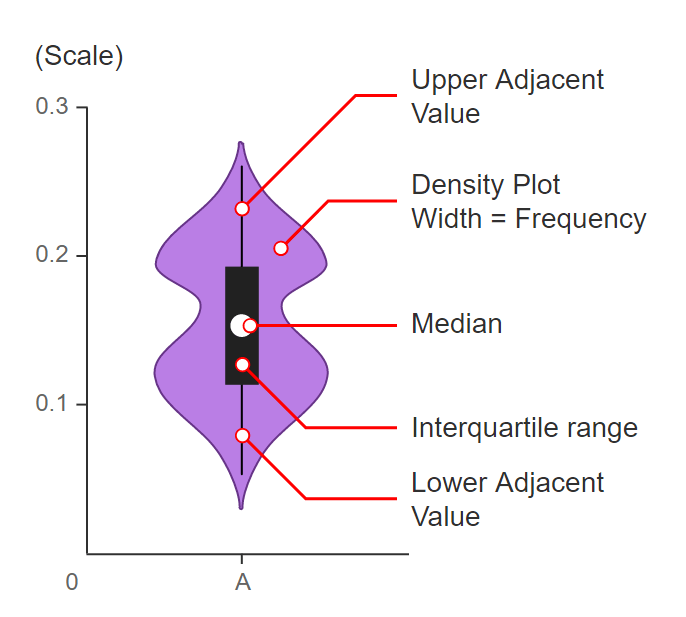
\includegraphics[width=0.5\linewidth]{houslovy_graf_2.png}
    \caption{Houslový graf 2.}
\end{figure}

\subsubsection{Bodový graf}

\begin{compactitem}
    \item Klasický, jednoduchý.
    \item Pro prvotní náhled na data, odhalí nejvýraznější rysy.
    \item Lze kombinovat s regresí.
\end{compactitem}

\begin{figure}[H]
    \centering
    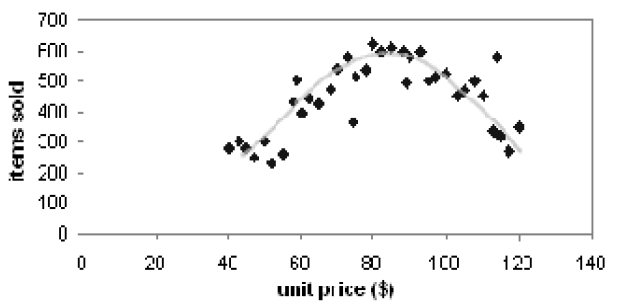
\includegraphics[width=0.75\linewidth]{bodovy_graf.png}
    \caption{Bodový graf.}
\end{figure}

\subsubsection{Sloupcový graf}

\begin{compactitem}
    \item Pro kategorické atributy.
\end{compactitem}

\begin{figure}[H]
    \centering
    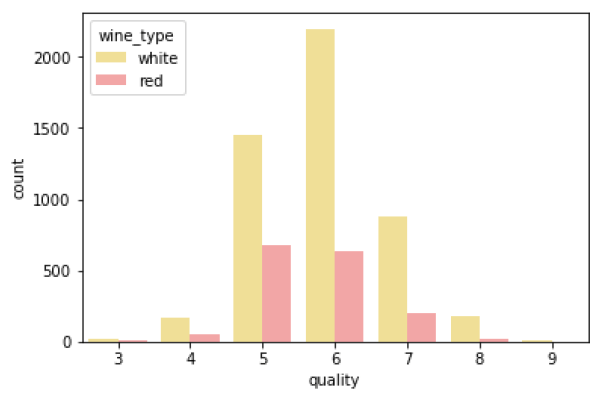
\includegraphics[width=0.75\linewidth]{sloupcovy_graf.png}
    \caption{Sloupcový graf.}
\end{figure}

%%%%%%%%%%%%%%%%%%%%%%%%%%%%%%%%%%%%%%%%%%%%%%%%%%%%%%%%%%%%%%%%%%%%%%%%%%%%%%%%

\section{Korelační analýza}

\begin{compactitem}
    \item Korelace (\textit{correlation}) popisuje vzájemný vztah mezi dvěma atributy (jak se vzájemně ovlivňují). Pokud se mezi dvěma atributy potvrdí korelace, je pravděpodobné, že jsou atributy na sobě závislé. Na základě toho však ještě nelze rozhodnout, zda jeden z~nich je příčinou a druhý následkem (korelace neimplikuje kauzalitu).

    \item Míra korelace je vyjadřována pomocí korelačních koeficientů, které nabývají hodnot z~intervalu $\langle-1,1\rangle$. Hodnota korelačního koeficientu $-1$ značí zcela nepřímou závislost (antikorelaci), tedy čím vyšších hodnot nabývá jeden atribut, tím nižších nabývá druhý. Hodnota korelačního koeficientu $+1$ značí zcela přímou závislost. Pokud je korelační koeficient roven 0 (nekorelovanost), pak mezi znaky není žádná statisticky zjistitelná lineární závislost. Avšak i při nulovém korelačním koeficientu na sobě veličiny mohou záviset, pouze tento vztah nelze vyjádřit lineární funkcí, a to ani přibližně.
\end{compactitem}

\subsection{Číselné vyjádření}

\begin{compactitem}
    \item Pro kvantitativní atributy: \begin{compactitem}
        \item \textbf{Pearsonův korelační koeficient} \begin{compactitem}
            \item Výpočet pomocí kovariace -- průměrná hodnota součinu vzdáleností jednotlivých atributů od průměrné hodnoty.

            \item A celé je ještě normalizované pomocí součinu směrodatných odchylek.

            \item Výsledek je z intervalu $(-1, 1)$ a vyjadřují pozitivní (přímá úměra) a negativní korelaci (nepřímá úměra).
        \end{compactitem}
        \begin{equation}
            {\displaystyle \rho _{X,Y}={\frac {\operatorname {cov} (X,Y)}{\sigma _{X}\sigma _{Y}}}}
        \end{equation}
    \end{compactitem}

    \item Pro kategorické atributy: \begin{compactitem}
        \item \textbf{Test dobré shody} \begin{compactitem}
            \item Je stanovena nějaká nulová (bázová) hypotéza a testem dobré shody se buďto vyvrací nebo nevyvrací.

            \item Rozdíl četností naměřených a očekávaných hodnot.

            \item Očekávané četnosti spočítáme dle nějakého rozdělení.

            \item Čím vyšší hodnota, tím vyšší pravděpodobnost, že jsou data korelovaná.
        \end{compactitem}
    \end{compactitem}
\end{compactitem}





\subsection{Vizuální techniky}

\begin{compactitem}
    \item Korelaci atributů vyhodnotíme na základě vizualizace, k tomu může sloužit např. \begin{compactitem}
        \item bodový graf,
        \item matice korelačních koeficientů s tepelnou mapou,
        \item matice bodových grafů.
    \end{compactitem}
\end{compactitem}

\begin{figure}[H]
    \centering
    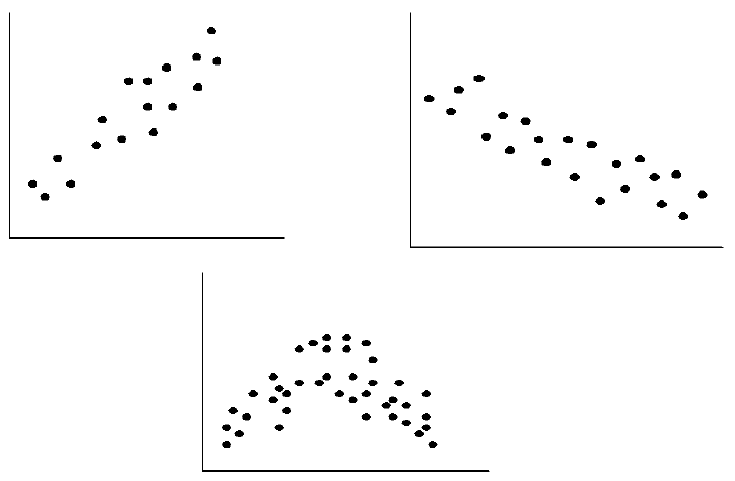
\includegraphics[width=0.5\linewidth]{korelace_bodovy_graf.png}
    \caption{Korelace v bodovém grafu.}
\end{figure}

\begin{figure}[H]
    \centering
    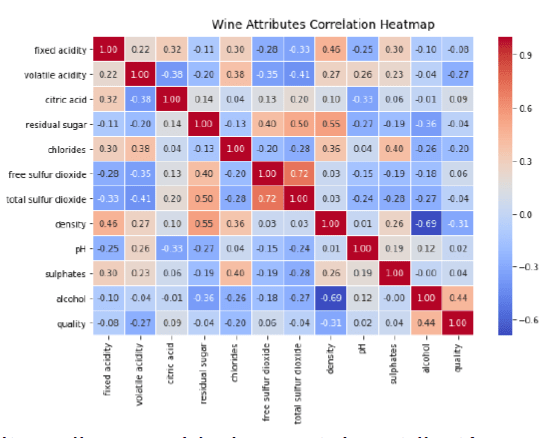
\includegraphics[width=0.8\linewidth]{korelace_teplotni_mapa.png}
    \caption{Korelace v matici korelačních koeficientů s teplotní mapou.}
\end{figure}

\begin{figure}[H]
    \centering
    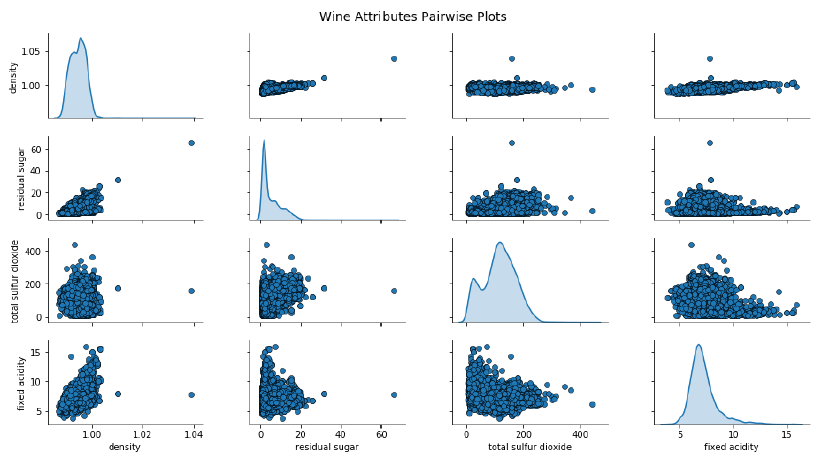
\includegraphics[width=1\linewidth]{korelace_matice.png}
    \caption{Korelace v matici bodových grafů.}
\end{figure}
